\documentclass[11pt]{article}
\usepackage[a4paper,margin=1in]{geometry}
\usepackage{amsmath}
\usepackage{graphicx}
\usepackage{float}
\usepackage{caption}
\usepackage[hidelinks]{hyperref}
\graphicspath{{figures/}}
\captionsetup{font=small}

\title{Generating Probabilistic Aerodrome Forecasts (TAFs) from\\
Numerical Weather Prediction: A Benchmark-Driven Model Review}
\author{Spanish airport network, 2020--2025}
\date{Working review}

\begin{document}
\maketitle

\begin{abstract}
We study whether machine learning can produce skilful, well-calibrated aerodrome forecasts
(TAFs) from numerical weather prediction (NWP) and recent observations, and beat the
official human-issued TAF. Using a strictly causal feature frame over 24 Spanish airports
(2.5\,M METARs, 0.25\,M TAFs; ERA5 reanalysis as a perfect-prognosis NWP proxy), we
benchmark a ladder of tabular models and a family of sequence/probabilistic models (GRU,
LSTM, Transformer, TCN, and a Temporal Fusion Transformer with quantile outputs) on a
frozen 2025 test set. The best model is a logistic \emph{stacked ensemble} of
\{MLP, gradient boosting, TFT\} reaching \textbf{BSS $+0.348$ / HSS $0.513$}, versus the
official TAF's $-0.108$, and it is near-perfectly calibrated. Driving PROB/TEMPO group
generation with it yields an operational TAF at BSS $+0.215$. Architecture is \emph{not}
the limiting factor: data scaling, model class, and the available feature set all plateau
near BSS\,$\approx +0.33$, indicating a data ceiling set by the ingested NWP fields and the
perfect-prognosis setup.
\end{abstract}

\section{Objective}
Predict, from information available at issue time $T_0$, the hourly aerodrome state over the
TAF validity window \emph{probabilistically}, so the model can be scored fairly against the
official TAF and drive automatic PROB/TEMPO change-group generation. The headline event is
\textbf{IFR-or-worse} (sub-instrument ceiling/visibility) --- operationally critical and
rare ($\sim$3.6\%).

\section{Data and setup}
Targets are METAR-derived vis, ceiling, wind and flight category at valid time $t$. Features
are strictly causal (enforced structurally): current and lagged METAR state ($t_0$,
$-1/-3/-6$\,h, with tendencies); ERA5 at $t$ and $T_0$ and the $T_0\!\to\!t$ tendency
(perfect-prognosis NWP); lead time; cyclical hour/day; static airport attributes. Splits are
temporal and blocked: train $<2024$, validation $=2024$, frozen test $=2025$; calibration is
fit on validation only.

\section{Metrics}
\textbf{BSS} (Brier Skill Score of $P(\text{IFR-or-worse})$ vs climatology; hedging-aware,
bootstrap CIs); \textbf{HSS} (categorical skill of the adverse decision at a
validation-tuned threshold); \textbf{reliability} (calibration). References: climatology
(BSS\,$=0$) and the official TAF (skyline). A key lesson: calibration (isotonic on
validation) is decoupled from the decision threshold; the raw class-weighted argmax must not
drive the forecast category.

\section{Models tested}
Baselines (persistence, climatology, official TAF); a tabular ladder (linear, gradient
boosting, a GPU multi-task MLP); sequence models (GRU, LSTM$+$attention, Transformer, TCN);
a TFT with quantile heads; and ensembles (linear blend, logistic stack). All deep models
share one framework, calibration contract and evaluation.

\section{Results}

\begin{figure}[H]\centering
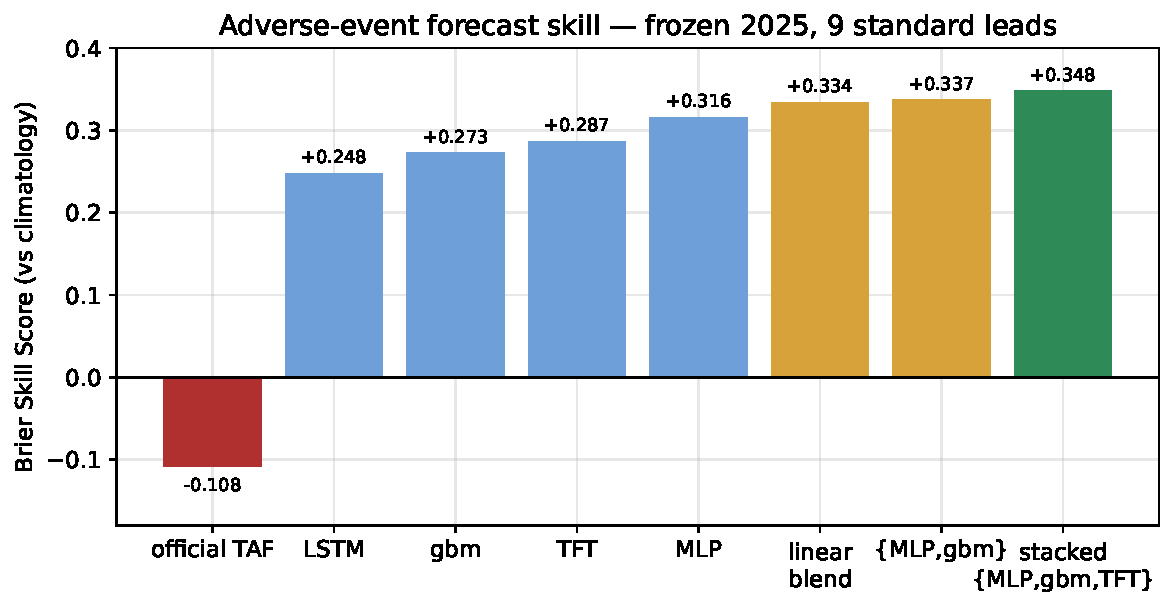
\includegraphics[width=0.92\linewidth]{fig1_model_comparison.pdf}
\caption{Adverse-event skill on the frozen 2025 test (9 standard leads). Every learned model
beats the official TAF ($-0.108$); ensembling leads.}
\end{figure}

\begin{figure}[H]\centering
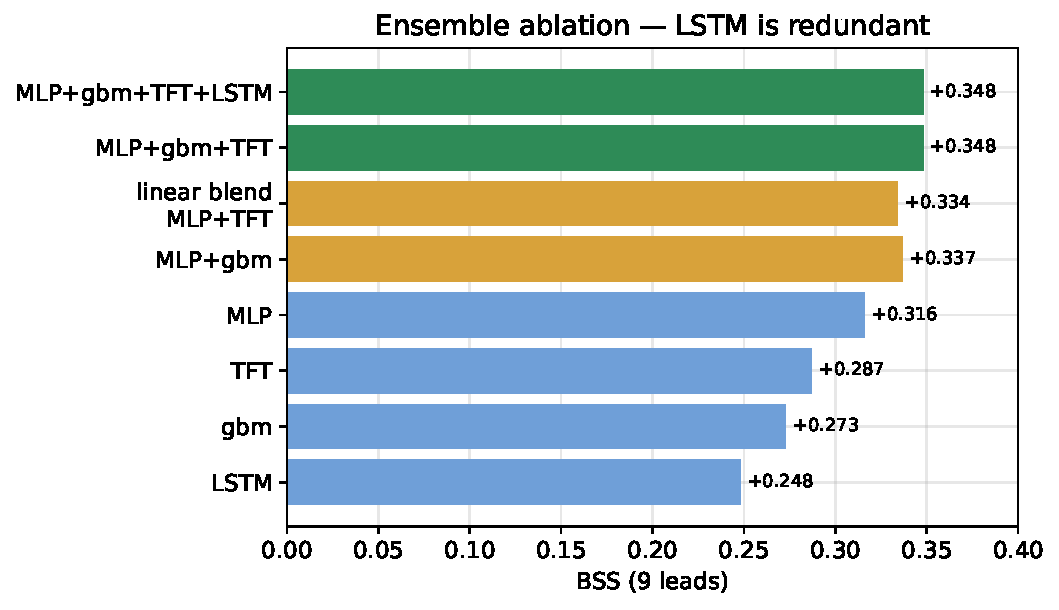
\includegraphics[width=0.80\linewidth]{fig6_ablation.pdf}
\caption{Stack ablation. \{MLP, gbm, TFT\} matches the full four-model stack (LSTM is
redundant); the TFT adds $+0.011$ over the tabular-only \{MLP, gbm\} stack.}
\end{figure}

\begin{figure}[H]\centering
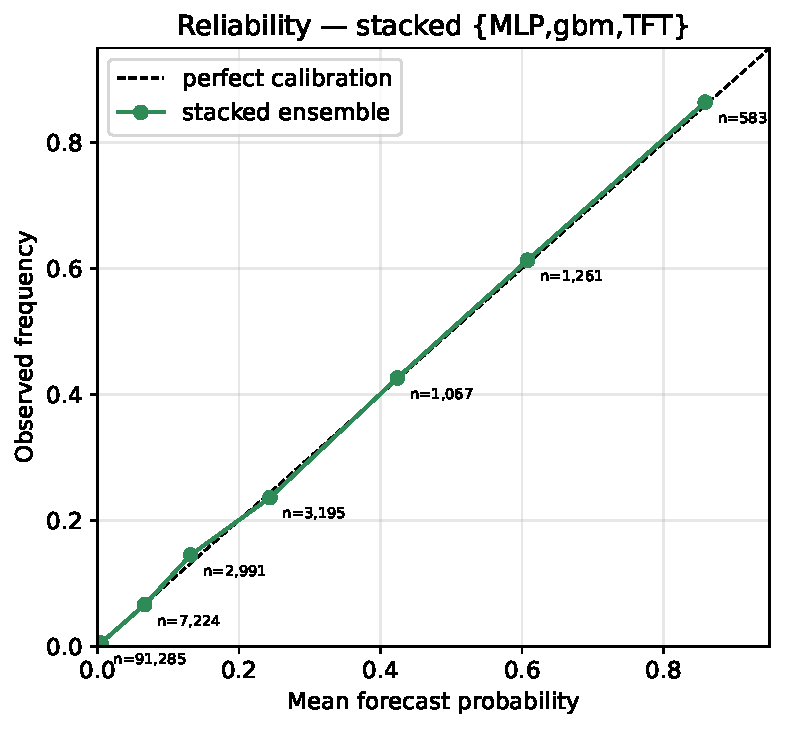
\includegraphics[width=0.55\linewidth]{fig2_reliability.pdf}
\caption{Reliability of the stacked ensemble: forecast probability matches observed
frequency to within $\pm0.01$.}
\end{figure}

\begin{figure}[H]\centering
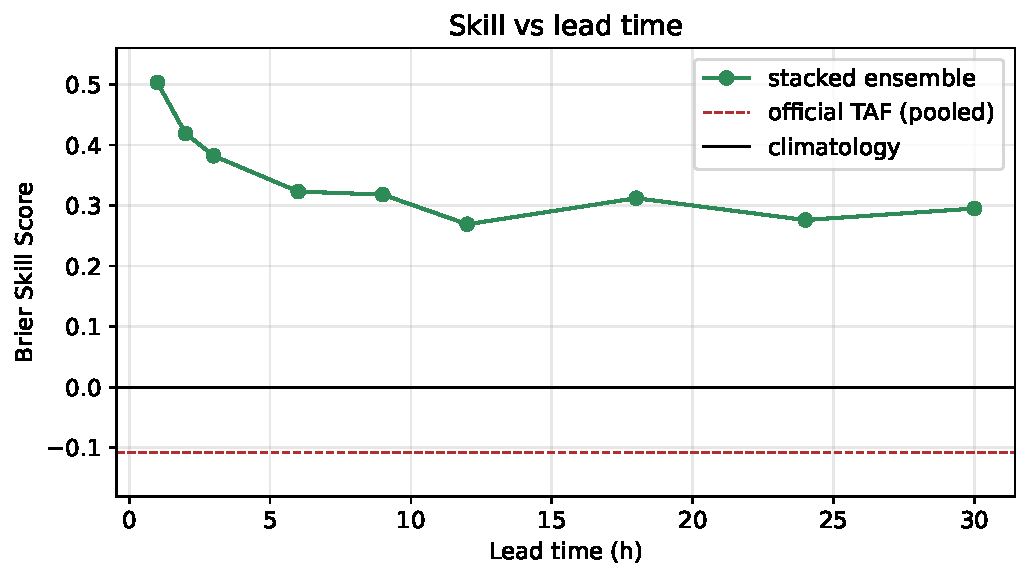
\includegraphics[width=0.70\linewidth]{fig3_skill_vs_lead.pdf}\\
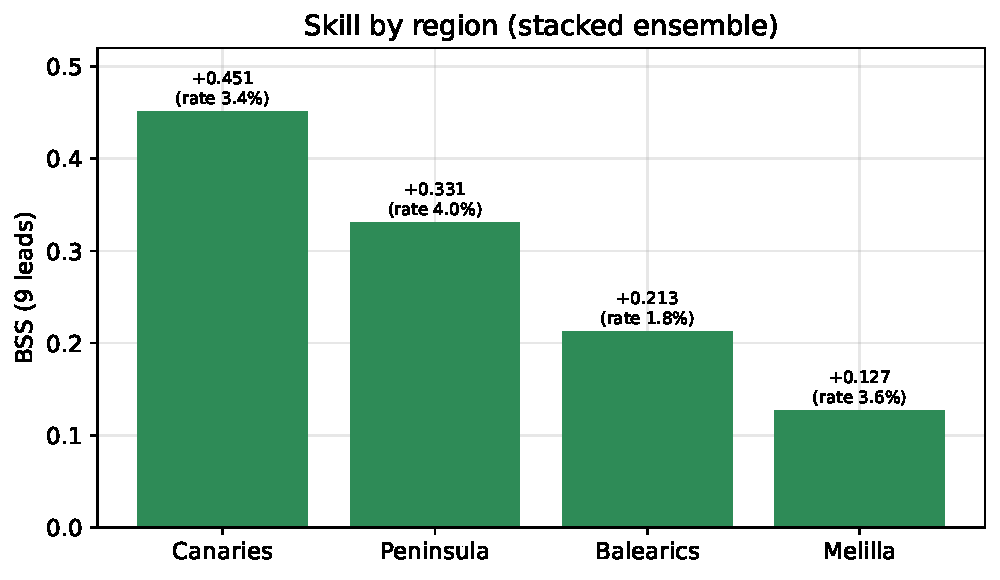
\includegraphics[width=0.70\linewidth]{fig5_region.pdf}
\caption{Skill vs lead time (top) and by region (bottom) for the stacked ensemble.}
\end{figure}

\begin{figure}[H]\centering
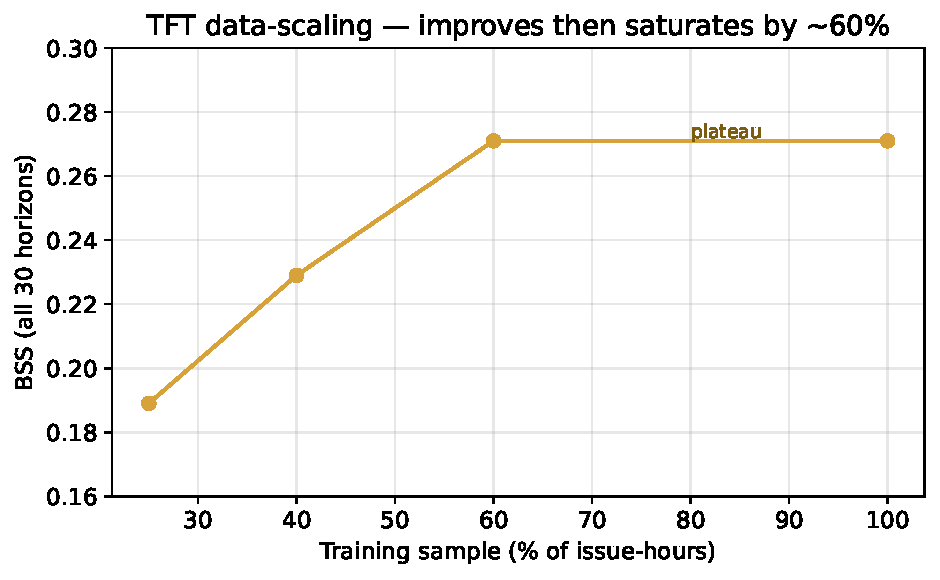
\includegraphics[width=0.64\linewidth]{fig4_scaling.pdf}
\caption{TFT data-scaling: skill improves then saturates by $\sim$60\% sample.}
\end{figure}

\section{Generating PROB/TEMPO TAFs}
The stacked $P(\text{adverse})$ is quantized to the TAF buckets (none / PROB30 / PROB40 /
firm) and combined with the TFT quantile element forecast to emit an hourly timeline with
PROB/TEMPO groups. The regenerated operational TAF scores BSS $+0.215$ (vs $-0.108$). The
TFT's visibility quantiles collapse to ``clear'' even at $q_{10}$, so adverse skill lives in
the calibrated category probability, not the element distribution; adverse groups use
category-representative conditions.

\section{Discussion and limitations}
Data volume, architecture and feature set all plateau near BSS\,$\approx +0.33$ --- a data
ceiling, not a modelling one. ERA5's cloud-layer split (the obvious ceiling/fog predictor)
was never ingested. The perfect-prognosis setup makes absolute skill optimistic; validation
against a genuine IFS/ECMWF reforecast is the credibility milestone. The highest-value next
step is richer / genuine-forecast NWP, not a larger network.

\section{Conclusion}
A calibrated, stacked ensemble of complementary model classes produces aerodrome forecasts
substantially more skilful and better calibrated than the official TAF
(BSS $+0.348$ vs $-0.108$) and drives a competitive operational PROB/TEMPO TAF.

\end{document}
